\documentclass[12pt, a4paper, twoside]{scrartcl}
 %---- Allgemeine Layout Einstellungen ------------------------------------------

% Für Kopf und Fußzeilen, siehe auch KOMA-Skript Doku
\usepackage[komastyle]{scrpage2}
\pagestyle{scrheadings}
\setheadsepline{0.5pt}[\color{black}]


%Einstellungen für Figuren- und Tabellenbeschriftungen
\setkomafont{captionlabel}{\sffamily\bfseries}
\setcapindent{0em}


%---- Weitere Pakete -----------------------------------------------------------
% Die Pakete sind alle in der TeX Live Distribution enthalten. Wichtige Adressen
% www.ctan.org, www.dante.de

% Sprachunterstützung
\usepackage[ngerman]{babel}

% Benutzung von Umlauten direkt im Text
% entweder "latin1" oder "utf8"
\usepackage[utf8]{inputenc}

% Pakete mit Mathesymbolen und zur Beseitigung von Schwächen der Mathe-Umgebung
\usepackage{latexsym,exscale,stmaryrd,amssymb,amsmath}

% Weitere Symbole
\usepackage[nointegrals]{wasysym}
\usepackage{eurosym}

% Anderes Literaturverzeichnisformat
%\usepackage[square,sort&compress]{natbib}

% Für Farbe
\usepackage{color}

% Zur Graphikausgabe
%Beipiel: \includegraphics[width=\textwidth]{grafik.png}
\usepackage{graphicx}

% Text umfließt Graphiken und Tabellen
% Beispiel:
% \begin{wrapfigure}[Zeilenanzahl]{"l" oder "r"}{breite}
%   \centering
%   \includegraphics[width=...]{grafik}
%   \caption{Beschriftung} 
%   \label{fig:grafik}
% \end{wrapfigure}
\usepackage{wrapfig}

% Mehrere Abbildungen nebeneinander
% Beispiel:
% \begin{figure}[htb]
%   \centering
%   \subfigure[Beschriftung 1\label{fig:label1}]
%   {\includegraphics[width=0.49\textwidth]{grafik1}}
%   \hfill
%   \subfigure[Beschriftung 2\label{fig:label2}]
%   {\includegraphics[width=0.49\textwidth]{grafik2}}
%   \caption{Beschriftung allgemein}
%   \label{fig:label-gesamt}
% \end{figure}
\usepackage{subfigure}

% Caption neben Abbildung
% Beispiel:
% \sidecaptionvpos{figure}{"c" oder "t" oder "b"}
% \begin{SCfigure}[rel. Breite (normalerweise = 1)][hbt]
%   \centering
%   \includegraphics[width=0.5\textwidth]{grafik.png}
%   \caption{Beschreibung}
%   \label{fig:}
% \end{SCfigure}
\usepackage{sidecap}
\usepackage{float}

% Befehl für "Entspricht"-Zeichen
\newcommand{\corresponds}{\ensuremath{\mathrel{\widehat{=}}}}
\newcommand{\folgt}{\ensuremath{\mathrel{\Rightarrow}}}
\newcommand{\equals}{\ensuremath{\mathrel{\Leftrightarrow}}}
\newcommand{\degree}{\ensuremath{\mathrel{^{\circ}}}}

\newcommand{\nn}{\nonumber}
\newcommand{\tn}[1]{\textnormal{#1}}
\newcommand{\D}{\ensuremath{\mathrel{\rm d}}}

\newcommand{\const}{\tn{const}}

\newcommand{\meter}{\ensuremath{\mathrel{\tn m}}}
\newcommand{\kilogramm}{\ensuremath{\mathrel{\tn{kg}}}}
\newcommand{\second}{\ensuremath{\mathrel{\tn s}}}
\newcommand{\sekunde}{\second}

\newcommand{\volt}{\ensuremath{\mathrel{\tn V}}}
\newcommand{\pascal}{\ensuremath{\mathrel{\tn{Pa}}}}
\newcommand{\coulomb}{\ensuremath{\mathrel{\tn C}}}
\newcommand{\newton}{\ensuremath{\mathrel{\tn N}}}
\newcommand{\liter}{\ensuremath{\mathrel{\tn l}}}
\newcommand{\celsius}{\ensuremath{\mathrel{\tn C}}}
\newcommand{\fahrenheit}{\ensuremath{\mathrel{\tn F}}}
\newcommand{\joule}{\ensuremath{\mathrel{\tn J}}}
\newcommand{\kelvin}{\ensuremath{\mathrel{\tn K}}}
\newcommand{\mol}{\ensuremath{\mathrel{\tn{mol}}}}
\newcommand{\gramm}{\ensuremath{\mathrel{\tn{g}}}}

\newcommand{\kilo}{\ensuremath{\mathrel{\tn k}}}
\newcommand{\hecto}{\ensuremath{\mathrel{\tn h}}}

\newcommand{\centi}{\ensuremath{\mathrel{ \tn c}}}
\newcommand{\milli}{\ensuremath{\mathrel{ \tn m}}}
\newcommand{\micro}{\ensuremath{\mathrel{ \tn\mu }}}



%\newcommand{}{\ensuremath{\mathrel{  }}}
%\newcommand{}{\ensuremath{\mathrel{  }}}
%\newcommand{}{\ensuremath{\mathrel{  }}}


\newcommand{\person}[1]{\textsc{#1}}

 \begin{document}
 %Titelseite
\begin{titlepage}
\centering
\textsc{\Large Anfängerpraktikum der Fakultät für
  Physik,\\[1.5ex] Universität Göttingen}

\vspace*{4.2cm}

\rule{\textwidth}{1pt}\\[0.5cm]
{\huge \bfseries
  Spezifische Wärme der Luft und Gasthermometer}\\[0.5cm]
\rule{\textwidth}{1pt}

\vspace*{3.5cm}

\begin{Large}
\begin{tabular}{ll}
Praktikanten: &  Silke Andrea Teepe\\
& Marcel Kramer\\
E-Mail: & \\
Betreuer: & Alexander Schmelev\\
\end{tabular}
\end{Large}

\vspace*{0.8cm}

\begin{Large}
\fbox{
  \begin{minipage}[t][2.5cm][t]{6cm} 
    Testat:
  \end{minipage}
}
\end{Large}

\end{titlepage}
\cleardoublepage
\tableofcontents
\cleardoublepage
\setcounter{page}{1}

\section{Einleitung}
\label{sec:einleitung}


\section{Theorie}
\label{sec:theorie}

\subsection{Gasthermometer}
Das Gasthermometer oder auch \person{Jolly}sche Luftthermometer ist ein Glaskolben der luftdicht an digitales Differenzdruckmessgerät angeschlossen ist. Das Messgerät zeigt nun die Druckdifferenz $\Delta p$ zwischen Umgebungsdruck $p_0$ und dem Druck $p$ im Glaskolben an. Im Kolben herscht folglich ein Druck von
\begin{align}
 p = p_0 + \Delta p \nn
\end{align}
Durch Temperaturänderungen ändert sich der Druck im Kolben und man kann mittels der in Kapitel \ref{subsec:theorie_eigenschaften_ideales_gas} beschrieben Formeln u.A. die Temperaturänderungen berechnen.

\subsection{Innere Energie eines Gases}
Die Moleküle in einem Idealen Gas werden als Punktförmig angesehen und es wird davon ausgegangen, dass es keine Wechselwirkungen innerhalb des Gases gibt.
Folglich ist die gesammte innere Energie $U$ des Gases die Summe der kinetischen Energie $E_{kin}$ der Moleküle. Mit der Temperatur $T$ als Maß der mittleren Energie der Moleküle gilt somit
\begin{align}
 E_{kin} = \frac{1}{2}\cdot m\cdot v^{2} = \frac{3}{2}\cdot k_B\cdot T \nn
\end{align}
mit der Bolzmannkonstante $k_B=1.381\cdot 10^{-23} \frac{\joule}{\kelvin}$
\\
Für einen realen Stoff gibt es neben den 3 Freiheitsgraden für Translation noch bis zu 3 Freiheitsgrade für Rotation bzw. 3 für Schwingungen.
Auf jeden dieser Freiheitsgrade entfällt somit die Energie
\begin{align}
 E = \frac{1}{2}\cdot k_B\cdot T \nn
\end{align}
Folglich hat ein Gas mit $N$ Molekülen und $f$ Freiheitsgraden die innere Energie
\begin{align}
 U = \frac{f}{2}\cdot N\cdot k_B\cdot T = \frac{f}{2}\cdot n\cdot R\cdot T \label{eq:U}
\end{align}
mit $n = \frac{N}{N_A}$ der Stoffmenge in $\mol$ und  der Gaskonstanten $R = N_A\cdot k_B$

\subsection{Eigenschaften eines Idealen Gases}
\label{subsec:theorie_eigenschaften_ideales_gas}
Der Zustand eines Idealen Gases kann durch die Größen Druck $p$, Volumen $V$ und Temperatur $T$ vollständig beschrieben werden.
Für eine Stoffmenge $n$ eines Idealen Gases gilt die Zustandsgleichung
\begin{align}
 p\cdot V = n\cdot R\cdot T \label{eq:zustandsgleichung}
\end{align}
Folglich gilt
\begin{align*}
 p &\propto T \tn{\;\; bei konstantem Volumen } V, \\
 V &\propto T \tn{\;\; bei konstantem Druck } p 
\end{align*}
und nach den Gesetzen von \person{Gay-Lussac} und \person{Boyle-Mariotte} gilt
\begin{align*}
 p\left(\vartheta\right) &= p_0\cdot\left[1+\beta\vartheta\right] \\
 V\left(\vartheta\right) &= V_0\cdot\left[1+\beta\vartheta\right]
\end{align*}
mit der Temperatur $\vartheta$ in $\degree\celsius$ und $\beta = \frac{1}{273.15 \degree\celsius}$ \footnote{Nach P. Schaaf (2014): ”Das Physikalische Praktikum”, Universitätsverlag Göttingen}.
Folglich hat ein Ideales Gas beim absoluten Nullpunkt von $-\frac{1}{\beta} = -273.15 \degree\celsius$ weder ein Volumen noch übt es einen Druck aus.

\subsection{Spezifische Wärme}
\subsubsection*{Isochore Temperaturänderung}
Der erste Hauptsatz der Wärmelehre besagt für die Änderung der inneren Energie $\Delta U$ eines abgeschlossenen Systems
\begin{align}
 \Delta U &= \Delta Q + \Delta W \label{eq:HS} \\
\equals \Delta Q &= \Delta U - \Delta W \nn 
\end{align}
mit $\Delta Q$ der hinzugefügten Wärmeenergie und $\Delta W = -p \Delta V$ der aufgebrachten Arbeit.
Bei einer isochoren Erwärmung, also bei $V = \const$ und damit $\Delta W = -p \Delta V = 0$, ist $\Delta U = \Delta Q$.
Aus Gleichung \eqref{eq:U} folgt für eine Temperaturänderung $\Delta T$ somit
\begin{align}
 \Delta Q = \Delta U = \frac{f}{2}\cdot n \cdot R \cdot \Delta T \label{eq:1}
\end{align}
Das Verhältnis
\begin{align}
 c_V &= \frac{\Delta Q}{\Delta T \cdot n} = \frac{f}{2} \cdot R \nn
%  \folgt \frac{c_V}{R} &= \frac{f}{2} \nn
\end{align}
bezeichnet die spezifische Wärmekapazität von einem Mol eines Gases (in $\frac{\joule}{\kelvin\cdot\mol}$).
Damit ergibt sich die Gleichung für die benötigte Energie einer isochoren Erwärmung um $\Delta T$
\begin{align}
 \Delta U = \left(\Delta Q\right)_V = n\cdot c_V \cdot \Delta T \label{eq:dU_V}
\end{align}

\subsubsection*{Isobare Temperaturänderung}
Wenn der Druck konstant beleibt aber nicht das Volumen, also eine isobare Erwärmung, muss zusätzlich noch die Volumenarbeit $p \cdot\Delta V$ aufgebracht werden.
Nach der Gleichung \eqref{eq:zustandsgleichung} ergibt sich
\begin{align}
 p\cdot\Delta V = n\cdot R\cdot \Delta T
\end{align}
Aus dem Hauptsatz folgt somit
\begin{align}
 \Delta Q &= \Delta U - \Delta W \nn\\
          &= \frac{f}{2} \cdot n\cdot R\cdot \Delta T + n\cdot R\cdot \Delta T \nn\\
          &= \left(\frac{f}{2}+1\right) \cdot n\cdot R\cdot \Delta T \nn\\
          &= c_p \cdot n\cdot \Delta T
\end{align}

Damit ergibt sich die Beziehung zwischen $c_p$ und $c_V$:
\begin{align}
 c_p = \left(\frac{f}{2}+1\right) \cdot R = c_V + R \nn
\end{align}

\subsubsection*{Gleichung für Freiheitsgrade}
Wenn keine Zustandgröße konstant beleibt gilt nach der Zustandsgleichung
\begin{align}
 \D \left(p\cdot V\right) &= n\cdot R\cdot \D T \nn\\
 \folgt \frac{\D p \cdot V + p \cdot \D V}{R} &= n \cdot \D T \label{eq:n_dT}
\end{align}
Aus den Gleichungen \eqref{eq:n_dT}, \eqref{eq:dU_V} und dem Hauptsatz folgt
\begin{align}
 \Delta Q &= \Delta U - \Delta W \nn\\
          &= c_V\cdot n\cdot \Delta T + p \cdot \Delta V \nn\\
          &= c_V \cdot \frac{\Delta p \cdot V + p \cdot \Delta V}{R} + p\cdot \Delta V \nn\\
 \folgt
 \Delta Q - p \cdot \Delta V &= \left(\Delta p \cdot V + p \cdot \Delta V\right)\cdot \frac{c_V}{R} \nn\\
 \folgt
 \frac{\Delta Q - p \cdot \Delta V}{\Delta p \cdot V + p \cdot \Delta V} &= \frac{c_V}{R} = \frac{f}{2} \label{eq:2}
\end{align}

\subsection{Kondensator}
Beim Aufladen eines Kondensator mit der Kapazität $C$ muss die Ladung $\Delta q$ die bereits aufgebaute Spannung $U = \frac{q}{C}$ überwinden. Dazu wird die Energie $\Delta E = \Delta q\cdot \frac{q}{C}$ benötigt.
Somit ist die Gesamtenergie $E$ im Kondensator der von $Q_0 = 0$ bis $Q_{max} = U \cdot C$ aufgeladen wird
\begin{align}
 E &= \int_{0}^{Q_{max}} \frac{q}{C}\cdot \D q \nn\\
   &= \frac{1}{2}\cdot\frac{Q_{max}^2}{C} \nn\\
   &= \frac{1}{2}\cdot C\cdot U^2
\end{align}



\section{Durchführung}
\label{sec:durchfuehrung}
\subsection{Gasthermometer}
\begin{figure}[h!]
	\centering
	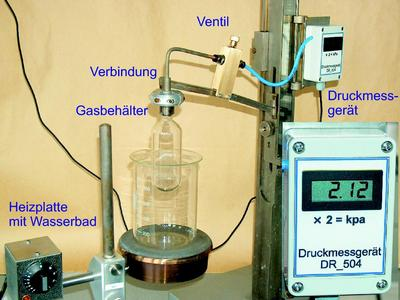
\includegraphics[scale=1]{Gasthermometer.png}
	\caption{Versuchsaufbau Gasthermometer\protect\footnotemark} 
\end{figure}
\footnotetext{https://lp.uni-goettingen.de/get/text/3643 Abb.3723}
Da das Druckmessgerät nicht in der Lage ist, negative  Druckdifferenzen zu erfassen, wird zunächst das Ventil geöffnet und im Glaskolben Luftdruck hergestellt. Mit Hilfe von Eiswasser wird dann der Kolben auf etwa $0\degree\celsius$ abgekühlt und anschließend das Ventil wieder verschlossen. Das Druckmessgerät sollte nun ca. $0.00\kilo\pascal$ anzeigen. \\
Nun bestimmt man den Druck $p_V \left( T \right)$ der Luft im Kolben für konstantes Volumen $V$ und Temperaturen zwischen $0\degree\celsius$ und $100\degree\celsius$, sowohl für Erwärmen, als auch Abkühlen des Kolbens. Dabei sollten Schritte von $\Delta T \le 5K $ gewählt werden. Um eine möglichste gleichförmige Temperaturänderung zu gewährleisten sollte das Wasserbad dauernd umgerührt werden.

\subsection{Spezifische Wärme der Luft}
\begin{figure}[h!]
	\centering
	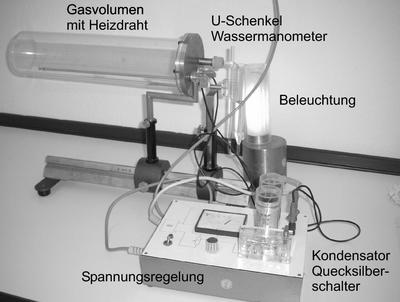
\includegraphics[scale=1]{SpezWaerme.png}
	\caption{Versuchsaufbau Spez. Wärme d. Luft \protect\footnotemark}
\end{figure}
\footnotetext{https://lp.uni-goettingen.de/get/text/3643 Abb.3724}
Ein Zylinder gefüllt mit Luft ist mit einem Wassermanometer verbunden. An dass Gasvolumen kann über einen Kondensator und einen Glühdraht eine spezifische Wärmemenge $Q$ abgegeben werden. Das Gasvolumen kann bei Vernachlässigung der Manometeränderung als konstant angesehen werden und somit die Druckänderung am Manometer abgelesen werden. \\
Der Kondensator wird aufgeladen und dann über den Heizdraht entladen. Dabei wird der maximale Ausschlag $\Delta p$ des Manometers abgelesen. Dieser wird für mehrfach für möglichst viele Spannungen zwischen 100V und 500V gemessen. Außerdem ist das Innenvolumen $V$ des Zylinders zu messen. \\
Während der Messung ist mit dem Ventil die Belüftungsöffnung des Zylinders zu verschließen und zwischen den Messungen beim Temperaturausgleich zu öffnen. Nach Beendigung der Messungen ist das Ventil geöffnet zurückzulassen.

\section{Auswertung}
\label{sec:auswertung}

\subsection{Gasthermometer}
Das Experiment wurde etwa 175$\meter$ über dem Meeresspiegel durchgeführt. Für den Umgebungsdruck nehmen wir daher $p_0=991,3\hecto\pascal$ an. Der Gesamtdruck $p$ im Glaskolben ergibt sich aus der Summe des Umgebungsdrucks und der Messwerte. $$p=p_0+p_K$$ Die Messwerte sind in den Abbildungen \ref{wplot} und \ref{kplot} zu sehen. Aufgrund des Gay-Lussac-Gesetzes kann ein linearer Zusammenhang angenommen werden. Der Ansatz für die Regression ist daher $p(T)=mT+b$. Der Ablesefehler des Druckmessgerätes ist gering und mit $0,2\kilo\pascal$ angenommen. Die Temperatur konnte nicht direkt im Glaskolben gemessen werden sondern musste in dem umgebenden Wasser gemessen werden. Wegen möglicher Temperaturunterschiede zwischen Wasser und Luft wird ein Gesamtfehler von $0,4\kilo\pascal$ verwendet.\\

Mit diesen Werten erhält man folgende Ergebnisse aus der linearen Regression

\begin{table} [h]
\centering
\begin{tabular}{r|c|c|c|c}
     & m & $\pm m$ & b & $\pm b$ \\
     \hline
    Aufwärmen &279,36 & 3,10 & 98861 & 172,4\\
     Abkühlen & 270,75 & 3,82& 99903& 197,3 \\
 \end{tabular} 
 \caption{\label{tab:}Ergebnisse der Regression mit Messfehlern}
\end{table}

Mit Hilfe des gewichteten Mittelwerts erhält man daraus
\begin{align*}
p(T)=\left(275,9\pm2,4\right)\frac{\kilo\pascal}{\degree\celsius}\,T+\left(99312\pm130\right)\kilo\pascal
\end{align*}
Der absolute Nullpunkt ergibt sich dann aus
\begin{align*}
p(T)\stackrel{!}{=}0\hspace{1.0cm}\Leftrightarrow\hspace*{1.0cm}T=-\frac{b}{m}=(-359,96\pm2,4)\degree\celsius
\end{align*}
wobei der Fehler durch die Gaußsche Fehlerfortpflanzung bestimmt wurde.

\begin{figure} [H]
\centering
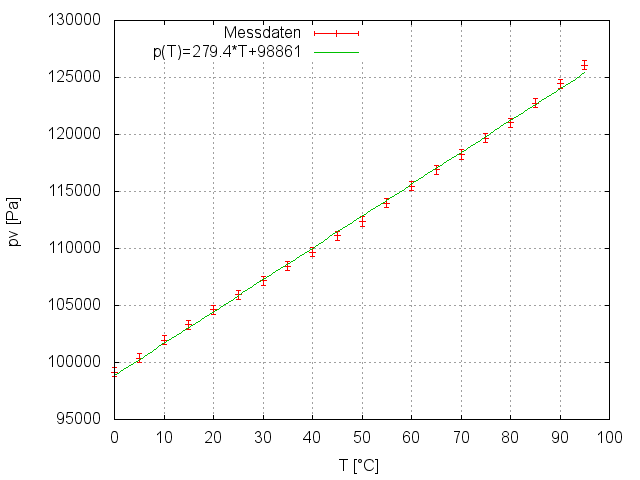
\includegraphics[scale=0.6]{waermen.png}
\caption{\label{wplot}Aufwärmen des Gasthermometers}
\end{figure}

\begin{figure} [H]
\centering
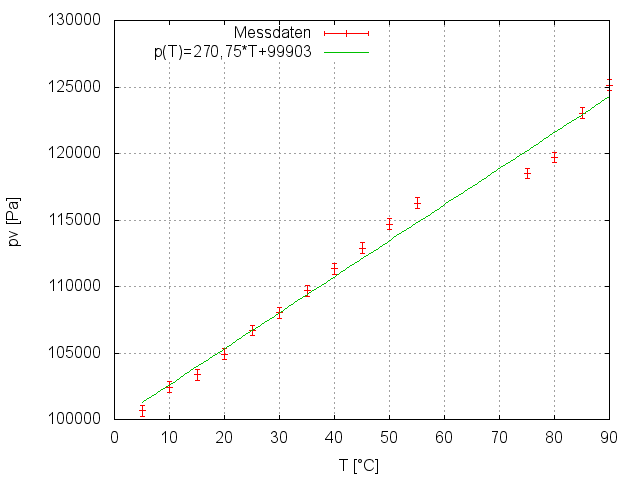
\includegraphics[scale=0.6]{abkuelen.png}
\caption{\label{kplot}Abkühlen des Gasthermometers}
\end{figure}




\subsection{Spezifische Wärme der Luft}
Für eine angelegte Spannung $U$ des Kondensators berechnet sich die elektrische Energie des Kondensators durch
\begin{align*}
\Delta Q=\frac{1}{2}\cdot C\cdot U^2
\end{align*}
Die Gesamtkapazität $C=2\cdot10\mu F$ ist die Summe der Kapazitäten der beiden Kondensatoren, die laut Praktikumsanleitung jeweils $10\mu F$ betragen. Der zugehörige Fehler ergibt sich aus der Fehlerfortpflanzung des Ablesefehlers $\sigma_U$ der mit $5\volt$ abgeschätzt ist. 
\begin{align*}
\sigma_{\Delta Q}=\sqrt{\left(\frac{\partial\Delta Q}{\partial U}\right)^2\cdot\sigma_U^2}=\sigma_U\cdot CU
\end{align*}
Die zugehörige Druckänderung ist durch
\begin{align*}
\Delta p=\rho g\Delta h=\rho g h_1\left(1+\frac{r_1^2}{r_2^2}\right)
\end{align*}
mit dem zugehörigen Fehler
\begin{align*}
\sigma_{\Delta p}=\sigma_h\rho g\left(1+\frac{r_1^2}{r_2^2}\right)=9.81\pascal
\end{align*}
gegeben. Aus der Praktikums anleitung erhält man die Werte für die Radien der Schenkel des Wasser-Manometers, die mit $r_1=2,0\milli\meter$ und $r_2=9,2\milli\meter$ angegeben sind sowie die Dichte von Wasser die $\rho_{H_2O}=1,0g$ beträgt. Das so berechnete Ergebnis ist in Abbildung \ref{druckplot} dargestellt, die exakten Zahlen Werte stehen zusammen mit dem Messdaten in Tabelle \ref{tab:spezwaerme}.


\begin{figure}[H]
\centering
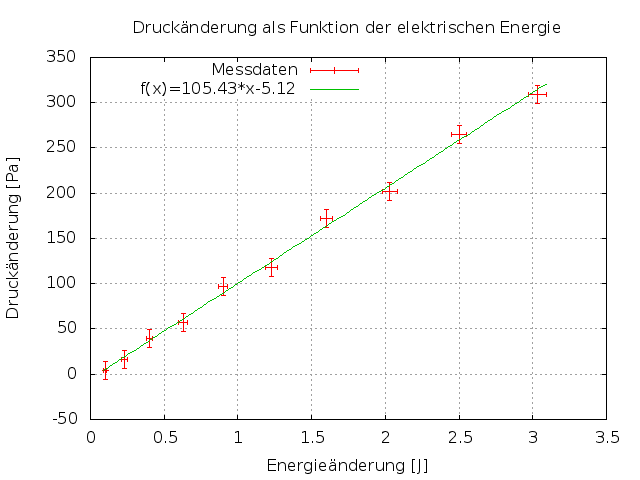
\includegraphics[scale=0.6]{druck.png}
\caption{\label{druckplot}Druckänderung als Funktion der elektrischen Energie}
\end{figure}


Um die Zahl der Freiheitsgerade zu bestimmen wird Formel \ref{eq:1} verwendet. Dazu wird das Volumen des Zylinders benötigt. Die Abmessung ergab für den Durchmesser $d=(8,9\pm0,2)\centi\meter$ und für die Länge $L=(40,0\pm0,2)\centi\meter$. Damit berechnet sich das Volumen zu \begin{align*}V=\pi \left(\frac{d^2}{2}\right)^2l=(0,0025\pm0,0001)m^3.\end{align*} Der Fehler wurde durch die Fehlerfortpflanzung ermittelt.
\begin{align*}
\sigma_V=\sqrt{\left(\frac{\partial V}{\partial d}\right)^2\cdot\sigma_d+\left(\frac{\partial V}{\partial l}\right)^2\cdot\sigma_l}=\sqrt{\left(\pi dl\right)^2\cdot\sigma_d+\left(\pi \frac{d^2}{2}\right)^2\cdot\sigma_l}
\end{align*}
Für den Luftdruck im Zylinder wird derselbe Raumdruck von $p=p_0=991,3hPa$ wie im Versuch \textit{Gasthermometer} verwendet.\\
Nun lassen sich die Freiheitsgerade $f$ gemäß
\begin{align*}
f=2\frac{\Delta Q-p\Delta V}{V\Delta p+p\Delta V}
\end{align*}
mit dem Fehler
\begin{align*}
\sigma_f&=\sqrt{\left(\frac{\partial f}{\partial \Delta p}\right)^2\sigma_{\Delta p}^2+\left(\frac{\partial f}{\partial \Delta Q}\right)^2\sigma_{\Delta Q}^2+\left(\frac{\partial f}{\partial \Delta V}\right)^2\sigma_{\Delta V}^2+\left(\frac{\partial f}{\partial V}\right)^2\sigma_{V}^2}\\
 &=\sqrt{\left(\frac{-2V(\Delta Q-p\Delta V)}{(V\Delta p+p\Delta V)^2}\right)^2\sigma_{\Delta p}^2+\left(\frac{2}{V\Delta p+p\Delta V}\right)^2\sigma_{\Delta Q}^2+\left(\frac{-2p(\Delta p+\Delta Q)}{(V\Delta p+p\Delta V)^2}\right)^2\sigma_{\Delta V}^2+}\\
 &\hspace{0.7cm}\overline{\left(\frac{-2\Delta(\Delta Q-p\Delta V)}{(V\Delta p+p\Delta V)^2}\right)^2\sigma_V^2}.
\end{align*}
Schließlich kann man die Molwärme $c_v$ aus der Zahl der Freiheitsgerade und der Gaskonstanten $R=8,314\frac{\joule}{\mol}$\footnote{[Dem I] Seite 266} mit Formel \ref{eq:2} bestimmen. Der Fehler ist
\begin{align*}
\sigma_{c_v}=\sqrt{\left(\frac{\partial c_v}{\partial f}\right)^2\sigma_f^2}=\frac{1}{2}R\sigma_f.
\end{align*}
Die Ergebnisse sind in Tabelle \ref{tab:fgrade} aufgeführt. Durch den gewichteten Mittelwert erhält man $f=7,35\pm0,21$ und $c_v=30,27\pm0,63\frac{\joule}{\mol\kelvin}$.










\section{Diskussion}
\label{sec:diskussion}

\subsection{Gasthermometer}
Der von uns gemessene Wert von  $T=(-362,08\pm2,4)\degree\celsius$ weicht um etwa $32$ Prozent vom Literaturwert von $-273,15\degree\celsius$\footnote{[Dem I] Seite 264} ab. Diese starke Abweichung ist wahrscheinlich hauptsächlich dadurch entstanden, dass der Glaskolben nicht vollständig im Wasser eingetaucht war. Außerdem ist unklar wie stark der tatsächliche Umgebungsdruck von dem angenommenen Wert abweicht.

\subsection{Spezifische Wärme der Luft}

Sauerstoff und Stickstoff verhalten sich so als ob sie fünf Freiheitsgerade besitzen. Der theoretische Wert für die Molwärme der Luft ist also $c_v=\frac{5R}{2}=20,785 \joule \mol^{-1} \kelvin^{-1}$ (der Anteil von Argon kann vernachlässigt werden). Vergleicht man die Zahl der tatsächlichen Freiheitsgraden mit unseren Messwerten fällt auf, dass besonders die Messungen bei $100 \volt$ und $150 \volt$ stark abweichen. Der Grund dafür kann eine kleine Abweichung der Nullposition der Skala mit der tatsächlichen Höhe des Wassers in der Ruheposition des Manometers seien. Diese verändert bei kleinen Spannungen den Messwert besonders stark. Die restlichen Werte liegen alle etwa 2,5 Freiheitsgerade über dem  tatsächlichen Wert. Es liegt also nahe, dass die Messung mit einem systematischen Fehler behaftet ist.





\section*{Literatur}

[Dem I] Demtröder Wolfgang, Experimentalphysik 1, 6. Auflage


\begin{table} [h]
\centering
\begin{tabular}{|r|c|c|c|c|}
	\hline
   $ U [\volt]$ & $ h [\milli\meter]$ & $ \Delta Q [\joule]$ & $ \sigma_{\Delta Q} [J]$ & $\Delta p [\pascal]$  \\
   \hline\hline
  $ 100$ & $0,4$ & $ 0,1$ & $ 0,010$ & $3,93$   \\
  $ 100$ & $0,4$ & $ 0,1$ & $ 0,010$ & $3,93$   \\
  $ 100$ & $0,4$ & $ 0,1$ & $ 0,010$ & $3,93$   \\ \hline
  $ 150$ & $1,6$ & $ 0,23$ & $ 0,015$ & $15,7$   \\
  $ 150$ & $1,8$ & $ 0,23$ & $ 0,015$ & $17,67$   \\
  $ 150$ & $1,6$ & $ 0,23$ & $ 0,015$ & $15,7$   \\ \hline
  $ 200$ & $4,0$ & $ 0,4$ & $ 0,020$ & $ 39,26$   \\ 
  $ 200$ & $4,0$ & $ 0,4$ & $ 0,020$ & $ 39,26$   \\
  $ 200$ & $4,0$ & $ 0,4$ & $ 0,020$ & $ 39,26$   \\ \hline
  $ 250$ & $6,0$ & $ 0,63$ & $ 0,025$ & $ 58,89$   \\
  $ 250$ & $5,6$ & $ 0,63$ & $ 0,025$ & $ 54,96$   \\
  $ 250$ & $6,0$ & $ 0,63$ & $ 0,025$ & $ 58,89$   \\ \hline
  $ 300$ & $10,0$ & $ 0,9$ & $ 0,030$ & $ 98,15$   \\
  $ 300$ & $10,0$ & $ 0,9$ & $ 0,030$ & $ 98,15$   \\
  $ 300$ & $9,6$ & $ 0,9$ & $ 0,030$ & $ 94,22$   \\ \hline
  $ 350$ & $12,0$ & $ 1,23$ & $ 0,035$ & $ 117,78$   \\
  $ 350$ & $12,0$ & $ 1,23$ & $ 0,035$ & $ 117,78$   \\
  $ 350$ & $12,0$ & $ 1,23$ & $ 0,035$ & $ 117,78$   \\ \hline
  $ 400$ & $18,0$ & $ 1,6$ & $ 0,040$ & $ 176,66$   \\
  $ 400$ & $17,0$ & $ 1,6$ & $ 0,040$ & $ 166,85$   \\
  $ 400$ & $17,6$ & $ 1,6$ & $ 0,040$ & $ 172,74$   \\ \hline
  $ 450$ & $21,6$ & $ 2,03$ & $ 0,045$ & $ 212,00$   \\
  $ 450$ & $20,0$ & $ 2,03$ & $ 0,045$ & $ 196,29$   \\
  $ 450$ & $20,0$ & $ 2,03$ & $ 0,045$ & $ 196,29$   \\ \hline
  $ 500$ & $28,0$ & $ 2,5$ & $ 0,050$ & $ 274,81$   \\
  $ 500$ & $27,0$ & $ 2,5$ & $ 0,050$ & $ 265,00$   \\
  $ 500$ & $26,0$ & $ 2,5$ & $ 0,050$ & $ 255,18$   \\ \hline
  $ 550$ & $33,0$ & $ 3,03$ & $ 0,055$ & $ 323,88$   \\
  $ 550$ & $31,6$ & $ 3,03$ & $ 0,055$ & $ 310,14$   \\
  $ 550$ & $30,0$ & $ 3,03$ & $ 0,055$ & $ 294,44$   \\ 
  \hline
 \end{tabular} 
 \caption{\label{tab:spezwaerme}Messdaten zum Versuch Spezifische Wärme der Luft}
\end{table}



\begin{table} [h]
\centering
\begin{tabular}{|r|c|c|c|c|}
	\hline
   $ U [\volt]$ & $ f $ & $ \sigma_f$ & $ c_v\left[\frac{\joule}{\mol\kelvin}\right]$ & $\sigma_{c_v}\left[\frac{\joule}{\mol\kelvin}\right]$  \\
   \hline\hline
  $ 100$ & $19,30$ & $ 46,18$ & $ 80,22$ & $191,99$   \\ \hline
  $ 150$ & $10,38$ & $ 6,02$ & $ 43,13$ & $25,03$   \\ \hline
  $ 200$ & $7,66$ & $ 1,89$ & $ 31,85$ & $7,84$   \\ \hline
  $ 250$ & $8,17$ & $ 1,38$ & $ 33,95$ & $5,74$   \\ \hline 
  $ 300$ & $6,98$ & $ 0,72$ & $ 29,01$ & $3,00$   \\ \hline
  $ 350$ & $7,82$ & $ 0,67$ & $ 32,52$ & $2,78$   \\ \hline 
  $ 400$ & $6,98$ & $ 0,42$ & $ 29,03$ & $ 1,76$   \\ \hline
  $ 450$ & $7,55$ & $ 0,39$ & $ 31,4$ & $ 1,63$   \\ \hline
  $ 500$ & $7,08$ & $ 0,29$ & $ 29,46$ & $ 1,21$   \\ \hline
  $ 550$ & $7,34$ & $ 0,26$ & $ 30,53$ & $ 1,09$   \\ \hline
  
 \end{tabular} 
 \caption{\label{tab:fgrade}Freiheitsgrade und Molwärme von Luft}
\end{table}

\end{document}
